% !TEX encoding = UTF-8
% !TEX TS-program = pdflatex
% !TEX root = ../../tesi.tex

\section{Vincoli dello stage}
Prima di iniziare con lo stage, è stato redatto, insieme al mio \textit{tutor} aziendale Fabio Pallaro, il piano di lavoro dove sono stati specificati i vincoli temporali e organizzativi. In seguito è stato approvato dal mio relatore, il professore Tullio Vardanega.

\subsection{Pianificazione temporale}
Lo stage si è svolto in una durata pari a 8 settimane, nel periodo che va dal 03-05-2021 al 25-06-2021, per un totale di 320 ore, ovvero 40 ore a settimana. Queste 8 settimane sono state divise in 3 periodi principali: il periodo di formazione, dove ho dovuto studiare i principi alla base delle varie \textit{blockchain} che sono andato ad utilizzare, con i relativi linguaggi di programmazione per la stesura degli \textit{smart contract}; il periodo di sviluppo dove ho dovuto produrre i vari \textit{smart contract} e le relative integrazioni con il \textit{back-end}; il periodo di validazione, collaudo e presentazione del prodotto. \\

\noindent La pianificazione settimanale è la seguente: 
\begin{itemize}
  \item \textbf{Prima settimana (40 ore)}:
  \begin{itemize}
      \item incontro con persone coinvolte nel progetto per discutere i requisiti e le richieste relative al sistema da sviluppare;
      \item verifica credenziali e strumenti di lavoro assegnati;
      \item studio dei concetti generali riguardanti la \textit{blockchain}.
  \end{itemize}
  \item \textbf{Seconda settimana (40 ore)}:
  \begin{itemize}
      \item studio della \textit{blockchain} Ethereum.
  \end{itemize}
  \item \textbf{Terza settimana (40 ore)}:
  \begin{itemize}
      \item studio del linguaggio Solidity per la definizione di \textit{smart contract}.
  \end{itemize}
  \item \textbf{Quarta settimana (40 ore)}:
  \begin{itemize}
      \item studio e implementazione degli \textit{smart contract} per la gestione di NFT seguendo lo standard ERC721 su \textit{blockchain} Ethereum.
  \end{itemize}
  \item \textbf{Quinta settimana (40 ore)}:
  \begin{itemize}
      \item studio della \textit{blockchain} Hotmoka.
  \end{itemize}
  \item \textbf{Sesta settimana (40 ore)}:
  \begin{itemize}
      \item studio e implementazione degli \textit{smart contract} per la gestione di NFT seguendo gli standard Hotmoka.
  \end{itemize}
  \item \textbf{Settima settimana (40 ore)}:
  \begin{itemize}
      \item conclusione codifica;
      \item integrazione tra il \textit{back-end} e una delle due implementazioni sviluppate;
      \item stesura della documentazione relativa al periodo di codifica.
  \end{itemize}
  \item \textbf{Ottava settimana (40 ore)}:
  \begin{itemize}
      \item collaudo della soluzione e stesura della documentazione finale;
      \item incontro di presentazione della soluzione con gli \textit{stakeholders};
      \item \textit{live demo} del lavoro di stage.
  \end{itemize}
\end{itemize}

\begin{figure}[!h]
  \centering
  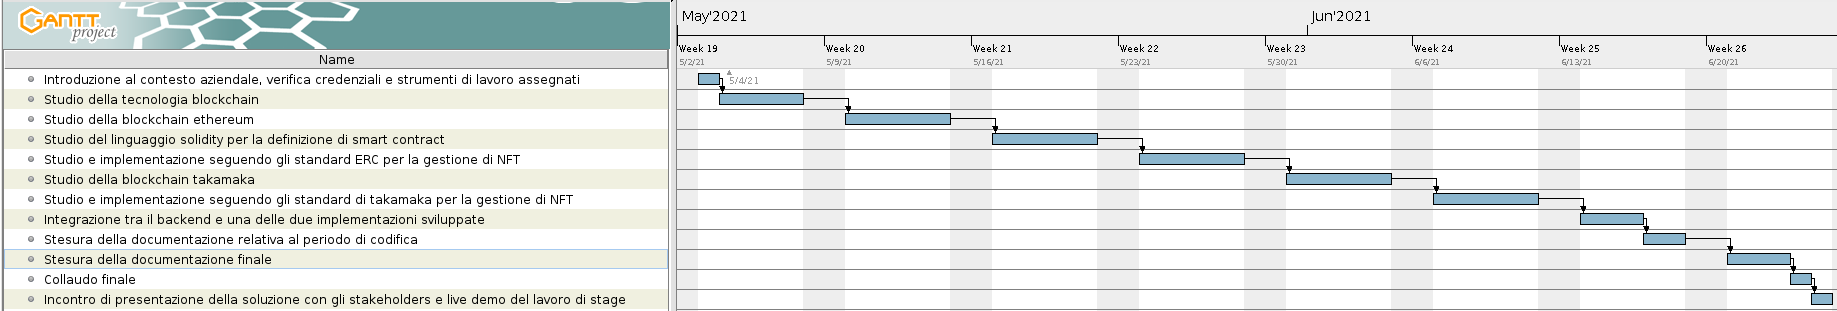
\includegraphics[width=\columnwidth]{capitolo2/gantt.png}
  \caption{Diagramma di Gantt relativo alla pianificazione dello stage}
\end{figure}

Per quanto riguarda la ripartizione oraria delle principali attività, qui si può vedere la tabella riassuntiva:
\begin{longtabu}{|c|X|}
	\hline

  \textbf{Durata in ore} & \textbf{Descrizione dell'attività} \\ \hline
  
	\textbf{160} & \textbf{Studio delle tecnologie} \\
  \textit{40} &
  Studio dei concetti generali riguardanti la \textit{blockchain} \\
  \textit{40} & 
  Studio della \textit{blockchain} Ethereum \\
  \textit{40} & 
  Studio del linguaggio Solidity per la definizione di \textit{smart contract} \\
  \textit{40} & 
  Studio della \textit{blockchain} Hotmoka \\

  \hline

  \textbf{80} & \textbf{Implementazione degli \textit{smart contract} per la gestione di NFT} \\ 
  \textit{40} & 
  Studio e implementazione degli \textit{smart contract} per la gestione di NFT seguendo lo standard ERC721 su \textit{blockchain} Ethereum \\
  \textit{40} & 
  Studio e implementazione degli \textit{smart contract} per la gestione di NFT seguendo gli standard Hotmoka \\
  
  \hline
  
  \textbf{24} & \textbf{Integrazione tra il backend e una delle due implementazioni sviluppate} \\
  \hline

  \textbf{40} & \textbf{Stesura documentazione} \\ 
  \textit{16} & 
  Stesura della documentazione relativa al periodo di codifica \\
  \textit{24} & 
  Stesura della documentazione finale \\

  \hline

  \textbf{16} & \textbf{Collaudo Finale}  \\ 
  \textit{13} & 
  Collaudo \\
  \textit{1} &
  Incontro di presentazione della piattaforma con gli \textit{stakeholders} \\
  \textit{2} & 
  Live demo del lavoro di stage \\
  \hline

  \textbf{Totale ore} & \multicolumn{1}{c}{\textbf{320}} \\ \hline

  \caption{Tabella riassuntiva delle ore per attività}
\end{longtabu}

\subsection{Vincoli organizzativi}
A causa della situazione pandemica ancora persistente, anche se in via di miglioramento, l'attività di stage è stata svolta in modalità mista. Sin dall'inizio dello stage è stato concordato con il mio \textit{tutor} aziendale, Fabio Pallaro, di fissare il lunedì come giorno obbligatorio di presenza in ufficio, in modo tale da poter eseguire lo \textit{sprint review}. 
Tutti gli altri giorni erano liberi e potevo scegliere personalmente se svolgere il lavoro in \textit{smart working}, oppure andare in ufficio. Per andare in ufficio dovevo prenotarmi minimo 2 giorni prima sulla piattaforma \textit{notion} e, nel caso ci fosse stato un numero considerevole di circa 10 persone gia prenotate, dovevo evitare di aggiungermi così da prevenire il superamento delle 15 persone massime permesse dalla legge.
Personalmente, oltre al lunedì, andavo in ufficio anche il venerdì in modo tale da avere un contatto più diretto ed efficiente con gli altri membri del gruppo che hanno lavorato al progetto NFTLab.\\

Per mantenere attiva la comunicazione con il mio \textbf{\textit{tutor} aziendale}, è stato creato un registro delle attività condiviso dove, giornalmente, ho scritto gli avanzamenti svolti nell'arco della giornata lavorativa. In seguito, ogni attività è stata verificata dal mio \textit{tutor} aziendale in modo tale da confermare la correttezza di quanto fatto. Per quanto riguarda il registro delle attività, ogni riga è stata organizzata nel seguente modo:
\begin{itemize}
  \item \textbf{Data}: data della giornata lavorativa interessata;
  \item \textbf{Descrizione}: breve descrizione dei progressi compiuti; 
  \item \textbf{Nota}: possibile nota del \textit{tutor} aziendale su quanto ho scritto nella descrizione;
  \item \textbf{\textit{Check} del \textit{tutor} aziendale}: spunta che conferma la correttezza degli avanzamenti realizzati.
\end{itemize}

\clearpage

\begin{figure}[!h]
  \centering
  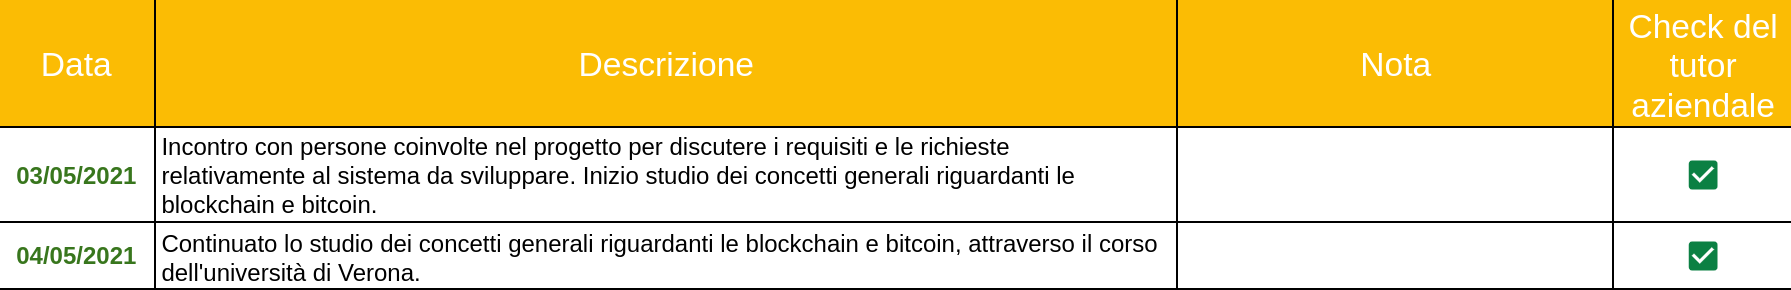
\includegraphics[width=\columnwidth]{capitolo2/registro-attivita.png}
  \caption{Estratto del registro delle attività}
\end{figure}

Per quanto riguarda la comunicazione con il mio \textbf{\textit{tutor} interno}, ho provveduto ad informarlo tramite \textit{email} ogni 5 giorni lavorativi, riassumendo gli avanzamenti compiuti durante la settimana e specificando se fossero o meno coerenti con la pianificazione settimanale concordata nel piano di lavoro. Nel caso in cui ci fosse stata l'opportunità di cambiamento della pianificazione settimanale, avrei dovuto sottoporre la modifica alla sua approvazione, specificando le varie motivazioni. \\

Durante il mio stage è stato fatto uso della metodologia \textbf{Scrum} in quanto è il metodo di sviluppo che viene adottato in tutti i progetti aziendali. Gli \textit{sprint} sono stati limitati ad una settimana e, come detto in precedenza, il lunedì era dedicato allo \textit{sprint review}. Questo mi ha permesso di analizzare e provare in prima persona la metodologia Scrum applicata in un ambito lavorativo e aziendale importante come lo è Sync Lab. \\

I \textbf{canali di comunicazione} utilizzati sono quelli che sono stati riportati in \ref{sec:tecnologie-utilizzate}. Più nello specifico è stato utilizzato:
\begin{itemize}
  \item \textbf{Discord}: tramite questa piattaforma è stato possibile rimanere in comunicazione con gli altri membri che stavano lavorando sul progetto NFTLab e con il mio \textit{tutor} aziendale, per esporgli qualsiasi mio dubbio e riferirgli i problemi che ho incontrato e non sono riuscito a risolvere anche dopo un periodo considerevole di tempo;
  \item \textbf{Google Meet}: utilizzato per partecipare alle varie riunioni o incontri urgenti svolte con gli \textit{stakeholders};
  \item \textbf{Trello}: \textit{scrum board} utilizzata per l'organizzazione degli \textit{sprint} settimanali;
  
  \clearpage
  \begin{figure}[!h]
    \centering
    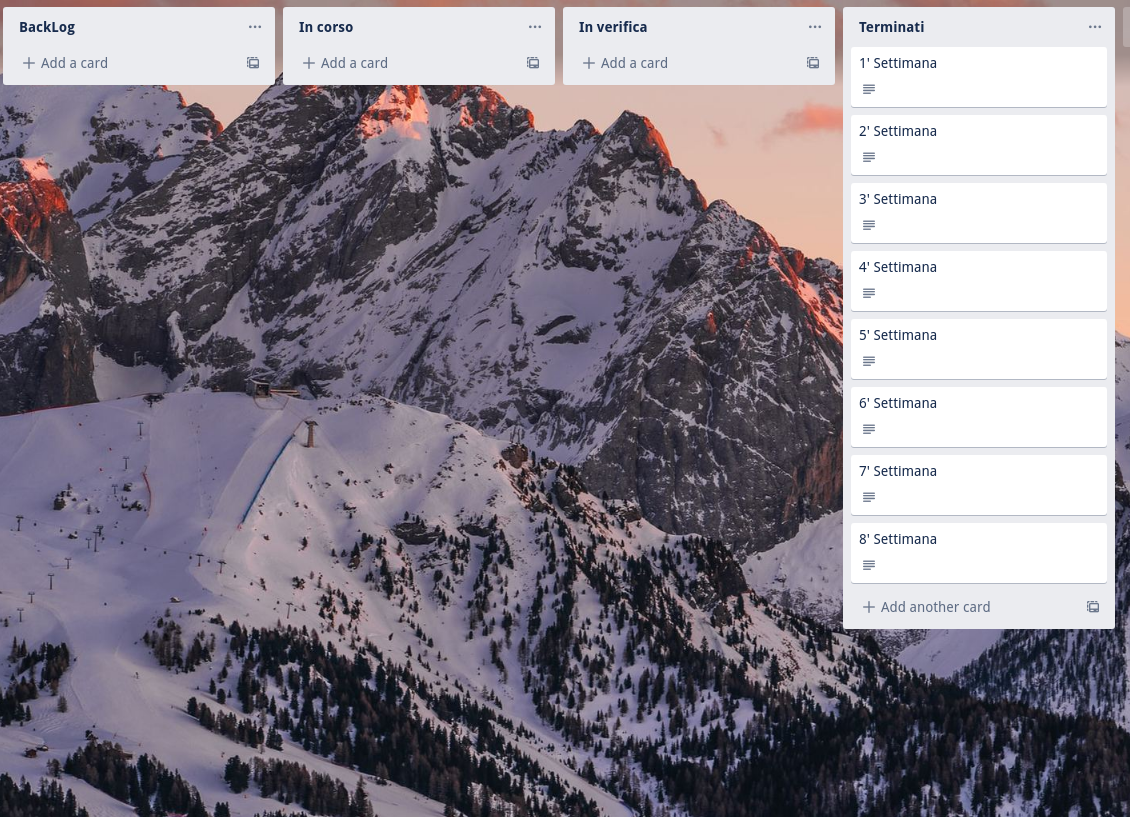
\includegraphics[width=0.8\textwidth]{capitolo2/trello-board.png}
    \caption{Gestione degli \textit{sprint} settimanali su Trello}
  \end{figure}

  \item \textbf{Notion}: impiegato, come già detto in precedenza, per la prenotazione della presenza in sede.
\end{itemize}

Per quanto riguarda la \textbf{gestione del codice}, non ci è stato imposto alcun vincolo da parte dell'azienda. Per questo motivo, in accordo con gli altri componenti del gruppo, è stata creata un'organizzazione sulla piattaforma GitHub dove sono raggruppate tutte le \textit{repository} e tutti gli artefatti prodotti.

% \clearpage

\begin{figure}[!h]
  \centering
  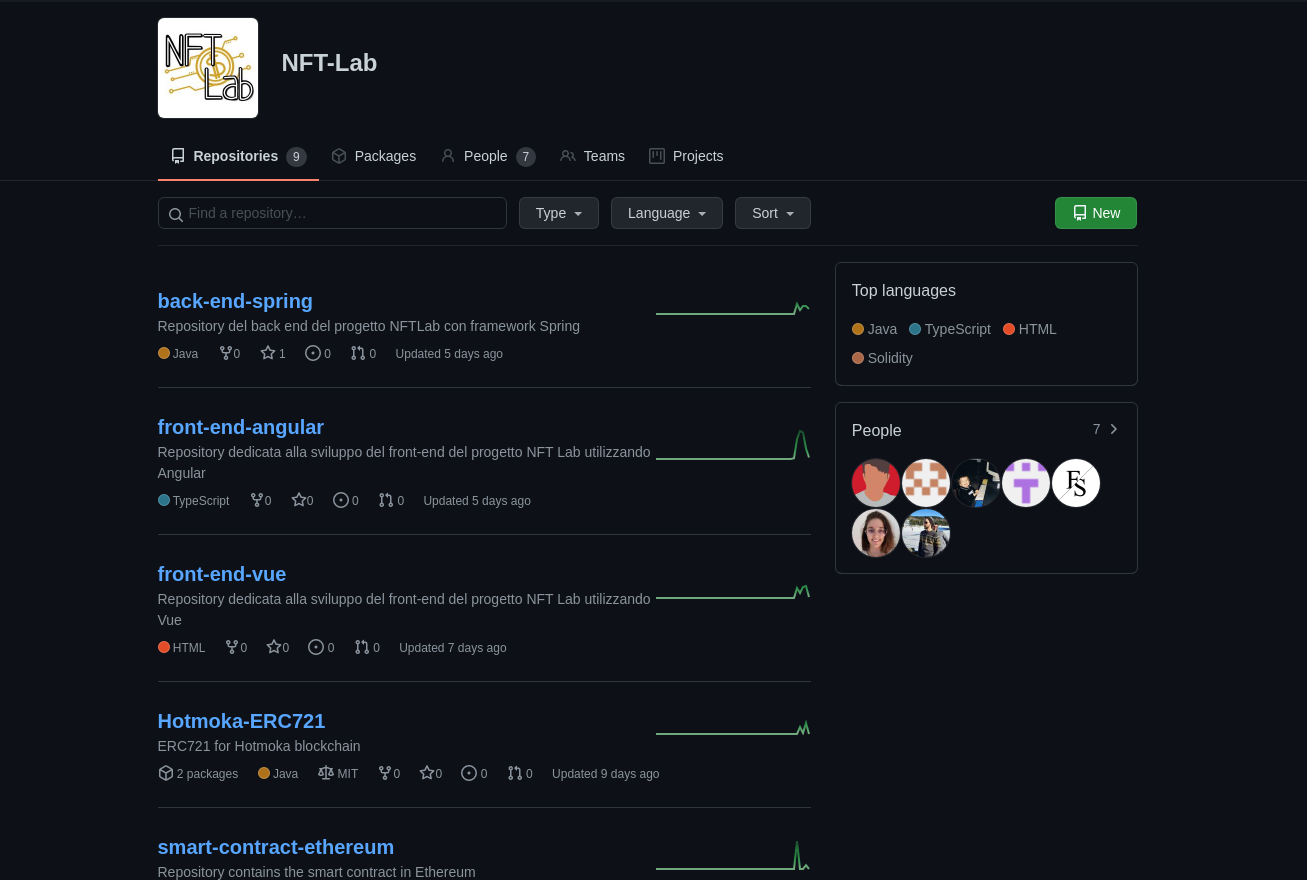
\includegraphics[width=0.8\textwidth]{capitolo2/github-organization.png}
  \caption{Organizzazione NFTLab su GitHub}
  \textbf{Fonte}: \href{https://github.com/NFT-Lab}{https://github.com/NFT-Lab}
\end{figure}
